\chapter{Lab System calls:系统调用实验}
\begin{introduction}
    \item 追踪系统调用
    \item 实现 Sysinfo 系统调用
    \item 系统调用的执行过程
    \item 增加系统调用的一般步骤
\end{introduction}

在上一个实验中,我们使用操作系统提供的各类系统调用完成了复杂的任务。在 Lab System calls 的实验中,我们会深入操作系统的内核,为 xv6 的系统调用添加一些功能,乃至添加新的系统调用。

\section{追踪系统调用}

为了方便对系统调用进行 debug ,我们引入一个新的系统调用 trace ,用以追踪(打印)用户程序使用系统调用的情况。该系统调用接受一个参数,被称为 mask (掩码),用以设置被追踪的系统调用:例如,若我们想要追踪 fork 系统调用,则需要调用 \lstinline{trace(1 << SYS_fork)} ,其中 \lstinline{SYS_fork} 是 fork 系统调用的编号。该进程调用过 \lstinline{trace(1 << SYS_fork)} 后,如果该进程后续调用了 fork 系统调用,调用 fork 时内核则会打印形如 \lstinline{<pid>: syscall fork -> <ret_value>} 的信息(但无需打印传入系统调用的参数)。

该实验提供了一个用户态程序用来方便我们测试 trace 功能,该用户态程序的源码在 \lstinline{user/trace.c} 。如果我们正确实现了 trace 系统调用,则使用 trace 用户程序的情况如下面的例子所示:

\begin{lstlisting}
$ trace 2147483647 grep hello README
4: syscall trace -> 0
4: syscall exec -> 3
4: syscall open -> 3
4: syscall read -> 1023
4: syscall read -> 966
4: syscall read -> 70
4: syscall read -> 0
4: syscall close -> 0
\end{lstlisting}

这个实验需要我们着手修改 xv6 的内核,但在修改内核之前,我们需要先将 \lstinline{$U/_trace} 加入到 \lstinline{Makefile} 中的 \lstinline{UPROGS} 环境变量中。此时如果直接运行 \lstinline{make qemu} ,则会无法通过编译,原因时我们还没有将 trace 系统调用加到 xv6 的用户态库和内核中。

按照下面的步骤将 trace 系统调用加入到户态库和内核中(具体的原理将在下文的小结中讨论):
\begin{enumerate}
    \item 在 \lstinline{user/user.h} 中的系统调用部分加入一行 \lstinline{int trace(int);} 作为 trace 系统调用在用户态的入口。
    \item 在 \lstinline{user/usys.pl} 中的系统调用部分加入一行 \lstinline{entry("trace");} 用以生成调用 \lstinline{trace(int)} 入口时在用户态执行的汇编代码(这段代码被称为 stubs )。
    \item 在 \lstinline{kernel/syscall.h} 中\lstinline{#define SYS_trace  22}为 trace 分配一个系统调用的编号。
\end{enumerate}

完成上述的工作后,应当能够通过 \lstinline{make qemu} 的编译,并且进入系统。由于我们还没有真正实现 trace 系统调用,故而如果我们在 xv6 的终端中执行 \lstinline{trace 32 grep hello README},进程会因为系统报 \lstinline{unknown sys call 22} 而被终止。

接下来我们可以开始真正实现 trace 系统调用了。首先,为了保存每个进程的 trace 的参数,我们需要在进程控制块中加入一个新的变量。查看 \lstinline{kernel/proc.h} ,找到进程的数据结构 \lstinline{struct proc},在其中加入一行 \lstinline{int tracemask;},如下所示:
\begin{lstlisting}[language=C,escapechar={!}]
struct proc {
  struct spinlock lock;

  // p->lock must be held when using these:
  enum procstate state;        
  void *chan;                  
  int killed;                  
  int xstate;                  
  int pid;                     

  // wait_lock must be held when using this:
  struct proc *parent;         

  // these are private to the process, so p->lock need not be held.
  uint64 kstack;               
  uint64 sz;                   
  pagetable_t pagetable;       
  struct trapframe *trapframe; 
  struct context context;      
  struct file *ofile[NOFILE];  
  struct inode *cwd;           
  char name[16];               
  !\hl{int tracemask; }!
};
\end{lstlisting}

为了将 \lstinline{trace(int)} 的参数保存到 \lstinline{struct proc} 中,我们需要在 \lstinline{kernel/sysproc.c} 中实现 \lstinline{sys_trace(void)} 函数,代码如下:

\begin{lstlisting}[language=C,escapechar={!}]
uint64
sys_trace(void)
{
  int mask;
  argint(0, &mask);
  myproc()->tracemask = mask;
  return 0;
}
\end{lstlisting}

其中, \lstinline{argint(0, &mask);} 用于获取用户传入系统调用的第一个参数,而 \lstinline{myproc()} 则返回当前进程控制块的指针,将其 \lstinline{tracemask} 赋值为获取到的参数即可。

然后我们需要修改 \lstinline{kernel/syscall.c} 中的 \lstinline{syscall(void)} ,使其能够根据 \lstinline{tracemask} 打印所需要的信息。首先定义一个字符串常量数组,保存各系统调用的名称:
\begin{lstlisting}[language=C,escapechar={!}]
const char *syscallnames[SYS_CALL_NUM + 1] = {
    "",
    "fork",
......
......
    "trace",
};
\end{lstlisting}

然后修改 \lstinline{syscall(void)} ,在调用系统调用后,增加如下 if 语句的内容:
\begin{lstlisting}[language=C,escapechar={!}]
void syscall(void)
{
...
    p->trapframe->a0 = syscalls[num]();

    if (p->tracemask >> num & 1)
    {
      printf("%d: syscall %s -> %d\n",
             p->pid, syscallnames[num], p->trapframe->a0);
    }
...
}
\end{lstlisting}

最后,为了让 fork 后的子进程能够继承 trace 的 \lstinline{tracemask} ,需要在 \lstinline{kernel/proc.c} 中的 \lstinline{fork(void)} 中加入复制 \lstinline{tracemask} 的语句,如下面的高亮代码所示:
\begin{lstlisting}[language=C,escapechar={!}]
int fork(void)
{
  int i, pid;
  struct proc *np;
  struct proc *p = myproc();

  // Allocate process.
  if ((np = allocproc()) == 0)
  {
    return -1;
  }

  // Copy user memory from parent to child.
  if (uvmcopy(p->pagetable, np->pagetable, p->sz) < 0)
  {
    freeproc(np);
    release(&np->lock);
    return -1;
  }
  np->sz = p->sz;

  // copy saved user registers.
  *(np->trapframe) = *(p->trapframe);
  // copy trace mask
  !\hl{np->tracemask = p->tracemask;}!
  // Cause fork to return 0 in the child.
  np->trapframe->a0 = 0;
  // increment reference counts on open file descriptors.
  for (i = 0; i < NOFILE; i++)
    if (p->ofile[i])
      np->ofile[i] = filedup(p->ofile[i]);
  np->cwd = idup(p->cwd);
  safestrcpy(np->name, p->name, sizeof(p->name));
  pid = np->pid;

  release(&np->lock);

  acquire(&wait_lock);
  np->parent = p;
  release(&wait_lock);

  acquire(&np->lock);
  np->state = RUNNABLE;
  release(&np->lock);

  return pid;
}
\end{lstlisting}


此时 trace 系统调用实现完成,编译并启动 xv6 后,在 shell 中运行 \lstinline{trace 32 grep hello README} ,即可看到预期的输出。

使用 xv6 实验自带的测评工具测评,在终端里输入 \lstinline{./grade-lab-syscall trace} ,即可进行自动评测,如下图所示:
\begin{figure}[H]
  \centering
  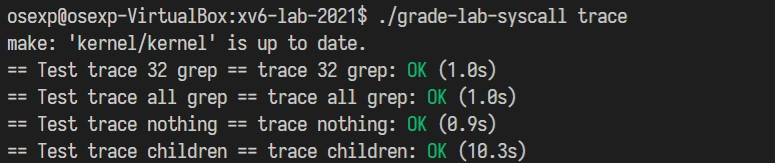
\includegraphics[width=0.8\textwidth]{syscall_trace.jpg}
  \caption{ trace 的测评结果}
\end{figure}
可见测试全部通过。

\section{实现 Sysinfo 系统调用}

常见的操作系统都会提供一些系统调用来帮助应用程序获取关于系统的信息,因而我们也被要求实现一个 sysinfo 系统调用,用于获取 xv6 运行时的信息。具体来说, xv6 已经为我们定义好了一个结构体 \lstinline{struct sysinfo} (在源码 \lstinline{kernel/sysinfo.h} )中,我们的 sysinfo 系统调用接受一个参数,即指向该结构体的指针,然后将对应的内容填入该结构体( \lstinline{freemem} 字段填写空闲的内存空间字节数, \lstinline{nproc} 字段填写状态为未使用( \lstinline{UNUSED} )的进程数)。 为了方便测试, xv6 还提供了一个用户程序 \lstinline{sysinfotest} ,当通过所有测试时该程序输出 \lstinline{sysinfotest: OK} 。

首先和上面类似,修改 \lstinline{Makefile} 中的 \lstinline{UPROGS} 环境变量,将 \lstinline{$U/_sysinfotest} 加入到其中。然后按照上面的流程添加 sysinfo 系统调用的入口,接着在 \lstinline{user/user.h} 中添加 \lstinline{struct sysinfo} 的声明:
\begin{lstlisting}[language=C,escapechar={!}]
    struct sysinfo;
    int sysinfo(struct sysinfo *);
\end{lstlisting}
然后可以通过编译。

为了获得空闲内存大小,我们需要在 \lstinline{kernel/kalloc.c} 实现一个函数。由于 xv6 管理内存空闲空间使用的是空闲链表,参照链表的结构后,只需遍历链表并计算数量,然后乘以页面大小即可。笔者的实现如下:
\begin{lstlisting}[language=C,escapechar={!}]
// Return the amount of free memory.
int getfreemem(void)
{
  int count = 0;
  struct run *r;

  acquire(&kmem.lock);
  r = kmem.freelist;
  while (r)
  {
    count++;
    r = r->next;
  }
  release(&kmem.lock);
  return count * PGSIZE;
}
\end{lstlisting}
\begin{theorem}[注意加锁] 
    当访问内核态的空闲链表时,由于可能出现并发读写的情况,故而我们需要先获取该数据结构的锁,然后再进行读取,最后释放该锁;否则可能读到“脏”的数据。使用下面的代码进行锁的获取和释放:
\begin{lstlisting}[language=C,escapechar={!}]   
acquire(&kmem.lock);
......
release(&kmem.lock);
\end{lstlisting}
\end{theorem}

统计空闲进程控制块的数量的函数的实现也类似,只是进程控制块是用静态数组管理的,故而只需要用一个循环遍历该数组即可。笔者在 \lstinline{kernel/proc.c} 中的实现如下:
\begin{lstlisting}[language=C]
// Return the number of non-UNUSED procs in the process table.
int getnproc(void)
{
  struct proc *p;
  int count = 0;
  for (p = proc; p < &proc[NPROC]; p++)
  {
    acquire(&p->lock);
    if (p->state != UNUSED)
    {
      count++;
      release(&p->lock);
    }
    else
    {
      release(&p->lock);
    }
  }
  return count;
}
\end{lstlisting}
\begin{theorem}[同样注意加锁] 
    访问内核态的数据结构时,谨慎起见总是要加锁。
\end{theorem}

由于虚拟存储机制的存在,内核态的页表与用户态的页表不同,而用户传入的地址是用户态的地址,故而剩下的问题就在于如何将内核态的数据复制到用户态的数据结构中。根据 xv6 实验手册 \footnote{\url{https://pdos.csail.mit.edu/6.828/2021/labs/syscall.html}} 的提醒,我们需要参考 \lstinline{kernel/sysfile.c} 中 \lstinline{sys_fstat()} 和 \lstinline{kernel/file.c} 中 \lstinline{filestat()} 的实现。在 \lstinline{filestat()} 中,有一行代码至关重要(下面高亮的一行):
\begin{lstlisting}[language=C,escapechar={!}]
// Get metadata about file f.
// addr is a user virtual address, pointing to a struct stat.
int
filestat(struct file *f, uint64 addr)
{
  struct proc *p = myproc();
  struct stat st;
  
  if(f->type == FD_INODE || f->type == FD_DEVICE){
    ilock(f->ip);
    stati(f->ip, &st);
    iunlock(f->ip);
    !\hl{if(copyout(p->pagetable, addr, (char *)\&st, sizeof(st)) < 0)}!
      return -1;
    return 0;
  }
  return -1;
}
\end{lstlisting}

此处的 \lstinline{copyout(p->pagetable, addr, (char *)&st, sizeof(st))} 接受进程的页表,并将内核态中的一段数据拷贝到进程内存空间中的地址处。有了这个函数,我们也可以用相同的方法将 \lstinline{struct sysinfo} 拷贝到用户态进程中,笔者在 \lstinline{kernel/sysproc.c} 中实现的 \lstinline{sys_sysinfo(void)} 如下所示:
\begin{lstlisting}[language=C]
extern int getnproc(void);
extern int getfreemem(void);
uint64
sys_sysinfo(void)
{
  struct proc *p = myproc();
  struct sysinfo st;
  uint64 addr; // user pointer to struct stat
  st.freemem = getfreemem();
  st.nproc = getnproc();
  if (argaddr(0, &addr) < 0)
    return -1;
  if (copyout(p->pagetable, addr, (char *)&st, sizeof(st)) < 0)
    return -1;
  return 0;
}
\end{lstlisting}

此时 sysinfo 系统调用实现完成,编译并启动 xv6 后,在 shell 中运行 \lstinline{sysinfotest} ,即可看到预期的输出:
\begin{lstlisting}
$ sysinfotest
sysinfotest: start
sysinfotest: OK
$ 
\end{lstlisting}

使用 xv6 实验自带的测评工具测评,在终端里输入 \lstinline{./grade-lab-syscall sysinfo} ,即可进行自动评测,如下图所示:
\begin{figure}[H]
  \centering
  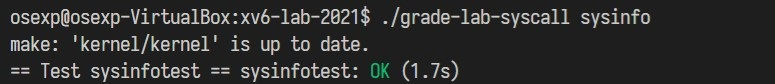
\includegraphics[width=0.8\textwidth]{syscall_sysinfo.jpg}
  \caption{ sysinfo 的测评结果}
\end{figure}
可见测试全部通过。

\paragraph*{实验结果} 在完成 Lab System calls 中的所有实验后,根据 MIT 6.S081 的传统,需要在实验目录下创建一个名为 \lstinline{time.txt} 文本文件,其中只包含一行,为完成该实验的小时数。然后在终端中执行 \lstinline{./grade-lab-syscall} ,即可对整个实验进行自动评分,笔者的结果如下:
\begin{figure}[H]
  \centering
  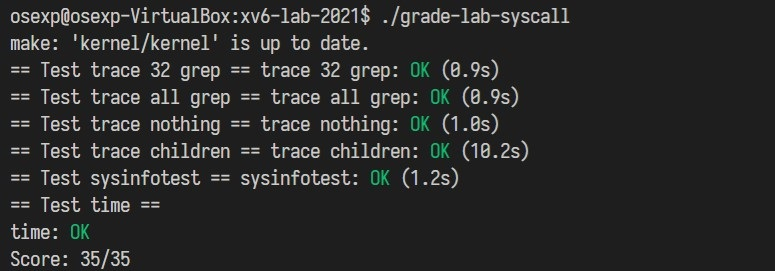
\includegraphics[width=0.8\textwidth]{syscall_grade.jpg}
  \caption{ Lab System calls 的测评结果}
\end{figure}
可见测试全部通过,得分为满分。

\section{小结:系统调用的执行过程}

通过上面的两个实验,我们能够大致了解一个系统调用发生的全过程。但实际上,上面的两个实验涉及到的内容并不细致,在这里笔者会以 sleep 系统调用为例,详细总结一个系统调用发生的各个阶段及其相关的细节。

首先准备实验环境,我们先从 \url{https://github.com/mit-pdos/xv6-riscv.git} 克隆下一个干净的 xv6 源码库,然后编写一个简单的 \lstinline{user/sleep.c},如下所示:
\begin{lstlisting}[language=C]
#include "kernel/types.h"
#include "kernel/stat.h"
#include "user/user.h"

int
main(int argc, char *argv[])
{
  sleep(10);
  exit(0);
}
\end{lstlisting}

将 \lstinline{$U/_sleep} 加入到 \lstinline{Makefile} 中的 \lstinline{UPROGS} 环境变量中,然后使用 \lstinline{make} 编译整个源码库。编译后除了会产生二进制文件外, xv6 的 \lstinline{Makefile} 还十分贴心地为我们生成了反汇编后的 \lstinline{user/sleep.asm} 文件,浏览该文件,可以看到如下的内容:
\begin{lstlisting}
user/_sleep:     file format elf64-littleriscv


Disassembly of section .text:

0000000000000000 <main>:
#include "kernel/stat.h"
#include "user/user.h"

int
main(int argc, char *argv[])
{
   0:	1141                	addi	sp,sp,-16
   2:	e406                	sd	ra,8(sp)
   4:	e022                	sd	s0,0(sp)
   6:	0800                	addi	s0,sp,16
  sleep(10);
   8:	4529                	li	a0,10
   a:	00000097          	auipc	ra,0x0
   e:	318080e7          	jalr	792(ra) # 322 <sleep>
  exit(0);
  12:	4501                	li	a0,0
  14:	00000097          	auipc	ra,0x0
  18:	27e080e7          	jalr	638(ra) # 292 <exit>
......
\end{lstlisting}
重点关注 \lstinline{sleep(10);} 的反汇编代码:
\begin{lstlisting}
......
  sleep(10);
   8:	4529                li	a0,10
   a:	00000097          	auipc	ra,0x0
   e:	318080e7          	jalr	792(ra) # 322 <sleep>
......
\end{lstlisting}

根据 RISC-V ABI ,寄存器 a0 用于存储函数的传入参数和返回值,故而该程序将立即数 10 加载到 a0 中,然后利用 \lstinline{auipc} 和 \lstinline{jalr} 两条指令跳转至 sleep 系统调用的函数体中。由于 \lstinline{jalr} 指令旁边的注释已经给出了 sleep 调用的地址,我们从该地址开始看:
\begin{lstlisting}
......
0000000000000322 <sleep>:
.global sleep
sleep:
 li a7, SYS_sleep
 322:	48b5                	li	a7,13
 ecall
 324:	00000073          	ecall
 ret
 328:	8082                	ret
......
\end{lstlisting}

这段代码即是 \lstinline{user/usys.S} 经汇编和链接后生成的代码,其中, \lstinline{li	a7,13} 将 sleep 的系统调用编号 13 载入到 a7 寄存器,此时的 a0 寄存器中仍然保存着我们传入 sleep 的参数 10 。然后程序执行 \lstinline{ecall} 进入内核态。下图展示了 \lstinline{ecall} 指令的机制\footnote{图片摘录自:\url{https://jborza.com/post/2021-04-21-ecalls-and-syscalls/}}:
\begin{figure}[H]
  \centering
  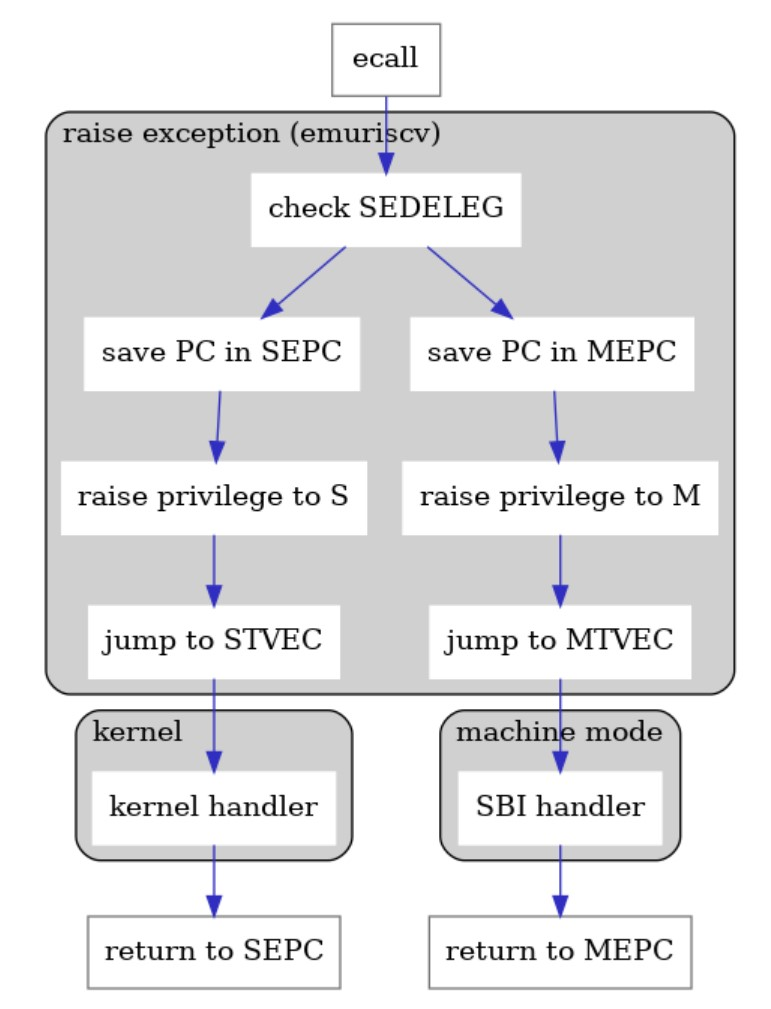
\includegraphics[width=0.6\textwidth]{syscall_ecall.jpg}
  \caption{ ecall 指令的机制}
\end{figure}

此时机器执行的是左侧的路径,即将当前的程序计数器 PC 保存到 SEPC 寄存器中,然后提升处理器的工作权限并跳转至 STVEC 所指向的代码处执行。此时 STVEC 所指向的代码即为 \lstinline{kernel/trampoline.S} 中的 \lstinline{.globl uservec},这段汇编代码保存用户态程序的各种寄存器到其 trapframe 中(此时的用户态程序便不再执行),恢复内核态的栈指针和页表,并跳转至 \lstinline{kernel/trap.c} 中的 \lstinline{usertrap(void)} 继续完成内核态的工作。

在 \lstinline{usertrap(void)} 中,获取了当前进程的控制块 \lstinline{struct proc *p = myproc();} 后,首先需要保存 \lstinline{ecall} 时保存到 SPEC 寄存器中的用户态 PC ,然后判断中断的种类。由 \lstinline{ecall} 引发的调用 syscall 的中断会使得 SCAUSE 的值被设为 8 ,故而会执行下面分支中的语句:
\begin{lstlisting}[language=C]
......
if(r_scause() == 8){
    // system call

    if(p->killed)
      exit(-1);

    // sepc points to the ecall instruction,
    // but we want to return to the next instruction.
    p->trapframe->epc += 4;

    // an interrupt will change sstatus &c registers,
    // so don't enable until done with those registers.
    intr_on();

    syscall();
......
\end{lstlisting}

该过程主要是将 trapframe 中保存的用户 PC 加 4 ,即指向 \lstinline{ecall} 的下一个指令,开启中断,并调用内核中系统调用的入口 \lstinline{syscall()} 。该入口在 \lstinline{kernel/syscall.c} 中被实现:
\begin{lstlisting}[language=C]
void
syscall(void)
{
  int num;
  struct proc *p = myproc();

  num = p->trapframe->a7;
  if(num > 0 && num < NELEM(syscalls) && syscalls[num]) {
    p->trapframe->a0 = syscalls[num]();
  } else {
    printf("%d %s: unknown sys call %d\n",
            p->pid, p->name, num);
    p->trapframe->a0 = -1;
  }
}
\end{lstlisting}

该函数获取了当前进程的控制块 \lstinline{struct proc *p = myproc();} 后,读取该进程企图调用的系统调用的编号:该编号在 \lstinline{user/usys.S} 中被放入 a7 寄存器中,然后 \lstinline{trampoline.S} 中的 \lstinline{uservec} 过程将 a7 寄存器中的值保存到了进程的 trapframe 中,此时使用 \lstinline{num = p->trapframe->a7;} 将其读出,稍作检查即可使用函数指针调用对应的实现。在本例子中,由于系统编号为 13 ,故调用的确实是 \lstinline{sys_sleep}:
\begin{lstlisting}[language=C]
uint64
sys_sleep(void)
{
  int n;
  uint ticks0;

  if(argint(0, &n) < 0)
    return -1;
  acquire(&tickslock);
  ticks0 = ticks;
  while(ticks - ticks0 < n){
    if(myproc()->killed){
      release(&tickslock);
      return -1;
    }
    sleep(&ticks, &tickslock);
  }
  release(&tickslock);
  return 0;
}
\end{lstlisting}

注意到在 \lstinline{kernel/sysproc.c} 中实现的 \lstinline{uint64 sys_sleep(void)} 并不接受参数,那之前用户态程序的参数如何传入到系统调用中呢?事实上,用户态程序将系统调用的参数保存在了 a0 ~ a5 着几个寄存器中,而这些寄存器在 \lstinline{uservec} 过程中都被保存到了进程的 trapframe 中(即都在内存中的进程控制块相关的数据结构中),故而只需要读取 trapframe 中对应的寄存器即可获得参数。读取寄存器的过程由一系列函数完成,如 \lstinline{int argint(int n, int *ip)} 、 \lstinline{static uint64 argraw(int n)} 等。

当 \lstinline{sys_sleep()} 完成了其工作后,返回至 \lstinline{syscall()} ,进而返回至 \lstinline{kernel/trap.c} 中的 \lstinline{usertrap(void)} ,此时执行 \lstinline{usertrapret();} 用于完成返回到用户态的工作:
\begin{lstlisting}[language=C]
void
usertrapret(void)
{
  struct proc *p = myproc();

  // we're about to switch the destination of traps from
  // kerneltrap() to usertrap(), so turn off interrupts until
  // we're back in user space, where usertrap() is correct.
  intr_off();

  // send syscalls, interrupts, and exceptions to trampoline.S
  w_stvec(TRAMPOLINE + (uservec - trampoline));

  // set up trapframe values that uservec will need when
  // the process next re-enters the kernel.
  p->trapframe->kernel_satp = r_satp();         // kernel page table
  p->trapframe->kernel_sp = p->kstack + PGSIZE; // process's kernel stack
  p->trapframe->kernel_trap = (uint64)usertrap;
  p->trapframe->kernel_hartid = r_tp();         // hartid for cpuid()

  // set up the registers that trampoline.S's sret will use
  // to get to user space.
  
  // set S Previous Privilege mode to User.
  unsigned long x = r_sstatus();
  x &= ~SSTATUS_SPP; // clear SPP to 0 for user mode
  x |= SSTATUS_SPIE; // enable interrupts in user mode
  w_sstatus(x);

  // set S Exception Program Counter to the saved user pc.
  w_sepc(p->trapframe->epc);

  // tell trampoline.S the user page table to switch to.
  uint64 satp = MAKE_SATP(p->pagetable);

  // jump to trampoline.S at the top of memory, which 
  // switches to the user page table, restores user registers,
  // and switches to user mode with sret.
  uint64 fn = TRAMPOLINE + (userret - trampoline);
  ((void (*)(uint64,uint64))fn)(TRAPFRAME, satp);
}
\end{lstlisting}


为了返回用户态, \lstinline{usertrapret();} 需要在关闭中断的条件下设置好进程的 trapframe 中的各数据项供 \lstinline{kernel/trampoline.S} 中的 \lstinline{uservec} 下次使用,然后还需要设置好处理器的工作模式、页表地址和用户态 PC ,最后使用函数指针的方式调用 \lstinline{kernel/trampoline.S} 中的 \lstinline{userret} ,恢复各寄存器,然后使用 \lstinline{sret} 指令回到用户态,并从用户态 PC 处开始执行。

此时的用户态程序从 \lstinline{ecall} 的下一个指令开始执行,恍如从一场梦中醒来,系统调用已经做完了其需要的事情。用户程序无法发觉操作系统内核进行了什么工作,颇有“地上一日,天上一年”的味道。

几乎所有的系统调用都与上面的过程类似,只有在内核态进行的工作有所不同。有一些涉及用户线程的系统调用(例如后文的定时器 alarm 系统调用),在返回用户态前会修改进程执行的上下文,但其返回用户态的工作总是由 \lstinline{kernel/trampoline.S} 中的 \lstinline{userret} 进行的。

\section{小结:增加系统调用的一般步骤}

通过上文对于系统调用执行过程的小结,我们很自然地能得出添加系统调用的一般步骤:
\begin{enumerate}
    \item 在 \lstinline{user/user.h} 中的系统调用部分加入系统调用在用户态的入口。
    \item 在 \lstinline{user/usys.pl} 中的系统调用部分加入在用户态执行的汇编代码( stubs )。
    \item 在 \lstinline{kernel/syscall.h} 中为系统调用分配一个系统调用的编号。
    \item 在内核代码中实现系统调用,包括设计对应的数据结构和函数等。
\end{enumerate}
从这个实验开始,我们便有能力对 xv6 的内核进行深度的改进,并在为其添加更多的特性的过程中学习现代操作系统的诸多概念。